\documentclass{article}

\usepackage{graphicx}

\begin{document}


\includegraphics[width=2.23958in,height=0.91667in]{media/image1.jpg}

\textbf{BHARATI VIDYAPEETH COLLEGE OF ENGINEERING,}

\textbf{NAVI MUMBAI}

A report on

\textbf{NAVIGATOR FOR VISUALLY IMPAIRED PERSON}

For

Major Project I (REV-2019 `C' Scheme)

of Final year, (BE SEM -- VII)

In

Electronics \& Telecommunication Engineering

\emph{Submitted By}

\begin{quote}
1. Nikhil Kanitkar A(23)

2. Dewoo Kudtarkar A(27)

3. Mandar Naik A(40)

4. Pranit Patil A(48)

\emph{Guide By}

Prof. S.S. Patil

2022-2023

\textbf{CERTIFICATE}
\end{quote}

This is to certify that the project report entitled \textbf{Navigator
For Visually Impaired Person} is a bonafide work of

\begin{quote}
1. Nikhil Kanitkar A(23)

2. Dewoo Kudtarkar A(27)

3. Mandar Naik A(40)

4. Pranit Patil A(48)
\end{quote}

Submitted to the University of Mumbai in partial fulfillment of the
requirement for the award of Major Project I (REV-2019 `C' Scheme) of
Final Year, (BE SEM-VII) in Electronics \& Telecommunication Engineering
as laid down by University of Mumbai during the academic year 2022-2023.

\textbf{Prof. S.S. Patil Prof. P.A.Kharade Dr. Sandhya Jadhav}

Name Of Guide Head Of Department Principal

\textbf{Project Report Approval}

This project report entitles "Navigator For Visually Impaired Person" by

1. Nikhil Kanitkar A(23)

2. Dewoo Kudtarkar A(27)

3. Mandar Naik A(40)

4. Pranit Patil A(48)

is approved for the degree of bachelors of engineering (Electronics and
Telecommunication engineering)

Examiner

1)------------------

2)------------------

Date: Place:

\textbf{ACKNOWLEDGMENT}

We are thankful to ``Bharati Vidyapeeth College of Engineering'' for
considering our project report and considering us through the various
stages of the project report. It gives us immense pleasure to express
our sincere gratitude of Prof. S.S. Patil for his guidance in selecting
the final year project report and also for providing us with all the
details.

We are deeply indebted to our respected Head of The Department of
Electronics and Engineering, Dr. P. A. Kharade, for giving us this
valuable opportunity to do this project and we express our heartily
thanks to them for their assistance without which it would have been
difficult in finishing this final year project report successfully.

We are also thankful to our respected Principal, Dr. Sandhya D. Jadhav.
We convey our deep sense of gratitude to all teaching and non-teaching
staff of The Department of Electronics and Telecommunication Engineering
for their constant encouragement, support and timely help throughout the
final year project report work.

\textbf{INDEX}

\begin{table}
\begin{tabular}{}
\toprule
\endhead
\begin{minipage}[t]{0.97\columnwidth}\raggedright
\textbf{Sr. No. Navigator For Visually Impaired Person Page Number}

\begin{enumerate}
\def\labelenumi{\arabic{enumi}.}
\item
  \begin{quote}
  \textbf{ABSTRACT.\ldots\ldots.\ldots\ldots\ldots\ldots\ldots\ldots\ldots\ldots\ldots\ldots\ldots\ldots\ldots\ldots\ldots\ldots\ldots\ldots\ldots....\ldots.......6}
  \end{quote}
\end{enumerate}

\textbf{2.
INTRODUCTION.\ldots\ldots\ldots.\ldots\ldots\ldots\ldots\ldots\ldots\ldots\ldots\ldots\ldots\ldots\ldots\ldots\ldots\ldots\ldots\ldots\ldots....7}

\textbf{3. LITERATURE
SURVEY.\ldots\ldots\ldots\ldots\ldots\ldots\ldots\ldots\ldots\ldots\ldots\ldots\ldots\ldots\ldots\ldots\ldots\ldots\ldots.8}

\textbf{4. PROPOSED
SYSTEM..\ldots\ldots\ldots\ldots\ldots\ldots\ldots..\ldots\ldots\ldots\ldots\ldots\ldots\ldots\ldots\ldots\ldots.\ldots.\ldots.9}

4.1 Algorithm \& Framework

4.2 Details Of Hardware

4.3 Details Of Software

4.4 Methodology

4.4.1 Research \& Survey

4.4.2 Block Diagram

4.4.3 Flow Chart

4.4.4 Output

\textbf{5. IMPLEMENTATION PLAN FOR NEXT
SEMESTER\ldots\ldots\ldots\ldots\ldots.\ldots.20}

\textbf{6.
CONCLUSION\ldots\ldots\ldots\ldots\ldots\ldots\ldots\ldots\ldots\ldots\ldots\ldots\ldots\ldots\ldots\ldots\ldots\ldots\ldots\ldots.\ldots\ldots\ldots.21}

6.1 Advantages

6.2 Limitations

6.3 Future Scope

\textbf{7. REFERENCES
\ldots\ldots\ldots\ldots\ldots\ldots\ldots\ldots\ldots\ldots\ldots\ldots\ldots\ldots\ldots\ldots\ldots\ldots\ldots\ldots.\ldots..\ldots.23}\strut
\end{minipage}\tabularnewline
\bottomrule
\end{tabular}
	\end{table}

\textbf{1. ABSTRACT}

According to WHO, India has 12 million visually impaired due to
uncorrected refractive error.

Several visually impaired people belong to the underprivileged
background and live in villages and tier 4 cities where they don't have
access to spectacles, but they are unaware this is correctable.

Navigator for Visually Impaired People refers to systems that can assist
or guide people with vision loss, ranging from partially sighted to the
blind, utilizing sound commands.

Creating a fusion of sensing technology and voice-based guidance system,
products can be developed which could give better results than
individual technology. The proposed system will be suitable to reduce
collision risks by enabling an impaired person to walk outdoors easily.

The suggested result includes a camera vision system to make an
independent operation for out-of-door navigation using the Internet of
things and create a good user experience to blind peoples.

\textbf{2. INTRODUCTION}

Recent studies on global health estimate that 217 million people suffer
from visual impairment, and 36 million from blindness. It has affected
their freedom threatened in terms of many everyday tasks, with the focus
being placed on those that involve moving through a strange environment.

In this regard, a navigation system's purpose is to provide users with
required and/or helpful data to get to a destination point. As we will
see, researchers working in this field have yet to find effective,
efficient, safe, and cost-effective technical solutions for both the
outdoor and indoor guidance needs of blind and visually impaired people.

This navigation system is designed for helping blind people to navigate
around safely. User does not need to move the white cane around to
detect obstacle like they do with the normal cane. Therefore a user can
easily walk with a white cane and continuously get information about
obstacles around with the help of sensors and IoT.

Much research is being conducted on building a navigation system for
visually impaired people. Several researchers address this challenge in
indoor and outdoor environments. However, most of these approaches have
limitations since this challenge involves many issues (e.g., accuracy,
and coverage).

\textbf{3. LITERATURE SURVEY}

\begin{longtable}[]{@{}llll@{}}
\toprule
\endhead
\textbf{Paper} & \textbf{Overview} & \textbf{Limitations} &
\textbf{Scope}\tabularnewline
Smart Cap -- Wearable Visual Guidance System For Blind, ISBN:
978-1-5386-2456-2. & The system uses Tensor Flow API for object
detecti-on. OpenCV helps in the image proc-essing operations. & Not
capable of recognizing objects near that person. & GPS module can be
introduced for improving efficie-ncy. Detection of objects at torso is
possible by placing sensor in belt, etc.\tabularnewline
Smart Assistive Navigation Devices for Visually Impaired People, ISBN:
978-1-7281-1322-7. & The paper presents a smart glass and a smart pair
of shoes by integrating various sensors with raspberry PI. & This device
is based on internet connectivity hence it is not reliable. & The
project can be made independent of internet so as it can work in region
with no internet facility.\tabularnewline
Smart Eye for Visually Impaired-An aid to help the blind people, ISBN:
978-1-5386-9471-8. & The project is a voice-enabled system that would
direct visually challenged people in their day-to-day work. & Difficult
to identify objects at ground level. & As the system is voice enabled,
Some mechanism to differentiate noise can improve the
system.\tabularnewline
Smart Stick For Blind People, ISBN: 978-1-7281-5197-7. & This paper
propo-sed a solution for blind people by using an the ultrasonic sensor
in the blind stick. & They can't detect obstructions that are hidden but
very dangerous for the blind such as downward stairs, holes, etc &
Instead of ultra-sonic sensor, some other sensor can be suggested to
make system more reliable.\tabularnewline
\bottomrule
\end{longtable}

\textbf{4. Proposed System}

\textbf{4.1 Algorithm \& Framework}

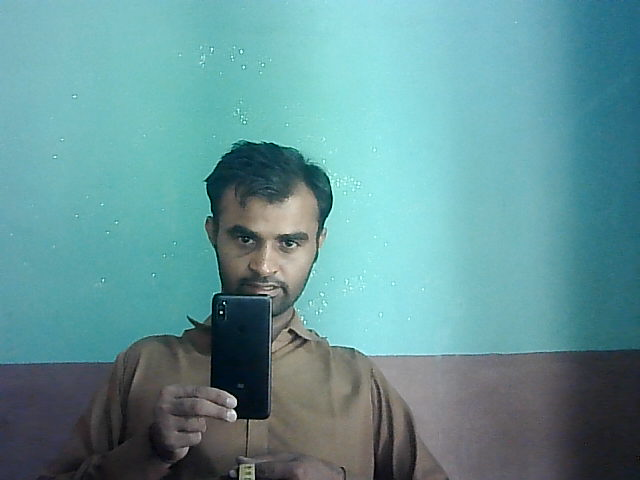
\includegraphics[width=2.925in,height=1.55347in]{media/image2.bmp}

The YOLO framework (You Only Look Once) deals with object detection
differently. It takes the entire image in a single instance and predicts
the bounding box coordinates and class probabilities for these boxes.
The biggest advantage of using YOLO is its superb speed -- it's
incredibly fast and can process 45 frames per second. YOLO also
understands generalized object representation.

The YOLO algorithm is important because of the following reasons:

\begin{enumerate}
\def\labelenumi{\arabic{enumi}.}
\item
  \begin{quote}
  {Speed}: This algorithm improves the speed of detection because it can
  predict objects in real time.
  \end{quote}
\item
  \begin{quote}
  {High accuracy}: YOLO is a predictive technique that provides accurate
  results with minimal background errors.
  \end{quote}
\item
  \begin{quote}
  {Learning capabilities}: The algorithm has excellent learning
  capabilities that enable it to learn the representations of objects
  and apply them in object detection.
  \end{quote}
\end{enumerate}

\textbf{4. Proposed System}

\textbf{4.2 DETAILS OF HARDWARE}

{Raspberry pi Zero 2W model}: Raspberry Pi Zero 2 W is perfect for IoT
projects this raspberry pi has a 1GHz quad-core 64-bit Arm Cortex-A53
CPU processor and 512MB SDRAM RAM and it supports 2.4GHz 802.11 b/g/n
wireless LAN, Bluetooth 4.2, Bluetooth Low Energy (BLE).

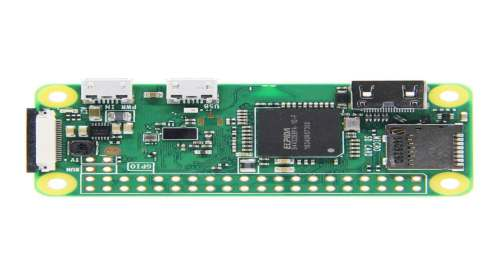
\includegraphics[width=3.46667in,height=1.95in]{media/1.jpg}

It has a Mini HDMI port, micro USB ports, and also having CSI-2 camera
connector.

{Raspberry PI Camera module}: This Raspberry PI Camera Module is a
custom-designed add-on for Raspberry PI. It attaches to Raspberry PI by
way of one of the two small sockets on the board's upper surface.

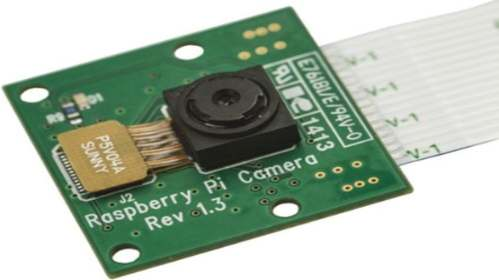
\includegraphics[width=3.46667in,height=1.95in]{media/2.jpg}

This interface uses the dedicated CSI interface, which was designed
especially for interfacing with cameras. The CSI bus is capable of
extremely high data rates. The 5MP camera module is perfect for small
Raspberry PI projects.

\textbf{4. Proposed System}

\textbf{4.2 DETAILS OF HARDWARE}

{Earbuds}: Earbuds are a pair of small loudspeaker drivers worn on or
around the head over a user's ears. We are using advanced Bluetooth 5.1.

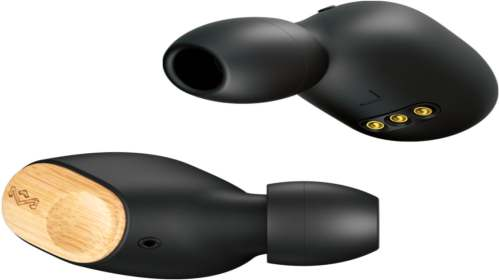
\includegraphics[width=3.46667in,height=1.95in]{media/3.jpg}

{ESP32}: ESP32 Development board is based on the ESP WROOM32 WIFI + BLE
Module. It's a low-footprint, minimal system development board powered
by the latest ESP-WROOM-32 module and can be easily inserted into a
solderless breadboard.

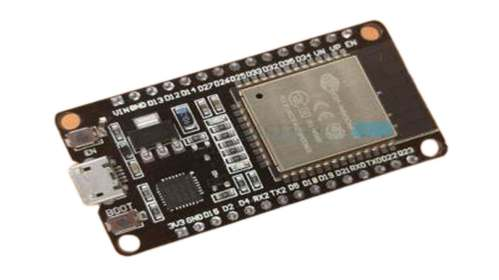
\includegraphics[width=3.46667in,height=1.95in]{media/4.jpg}

Including the USB-UART bridge, reset- and boot-mode buttons, LDO
regulator, and a micro-USB connector.

\textbf{4. Proposed System}

\textbf{4.2 DETAILS OF HARDWARE}

{Ultrasonic sensor (HC-SR04)}: This ultrasonic sensor module can be used
for measuring distance, object sensors, motion sensors, etc.

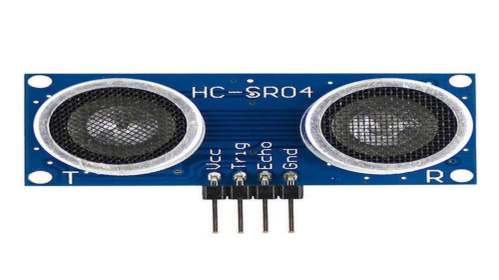
\includegraphics[width=3.46667in,height=1.95in]{media/5.jpg}

The high-sensitive module can be used with a microcontroller to
integrate with motion circuits to make robotic projects and other
distance, position \& motion-sensitive products. Detection distance: 2cm
-- 400cm (0.02M - 4.0M).

{Vibrator Motor}: Vibrator Motor is a shaftless vibration motor that is
fully enclosed with no exposed moving parts. Its small size (10 mm
diameter, 3.4 mm height) and shaftless design mean you can mount it on a
PCB.

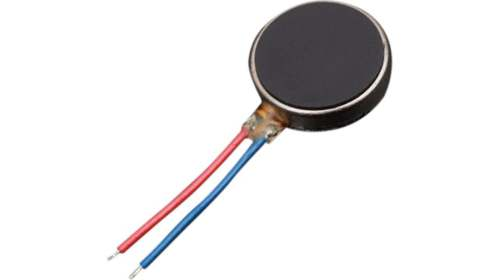
\includegraphics[width=3.46667in,height=1.95in]{media/6.jpg}

This tiny, button-type, vibrating motor shakes with a vibration
amplitude of 0.75g and draws approximately 60mA when 3V is applied to
its leads.

\textbf{4. Proposed System}

\textbf{4.2 DETAILS OF HARDWARE}

{Power bank}: We are using a power bank to power up the raspberry PI and
ESP32 both on an operating voltage of them and it is rechargeable.

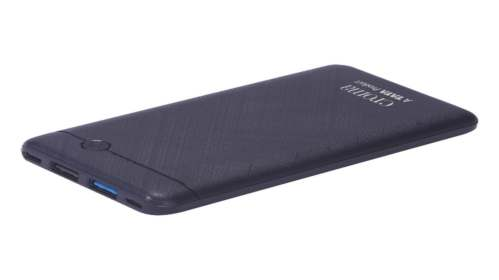
\includegraphics[width=3.46667in,height=1.95in]{media/7.jpg}

{Wires}: We are using single-strand wires for connecting the components.

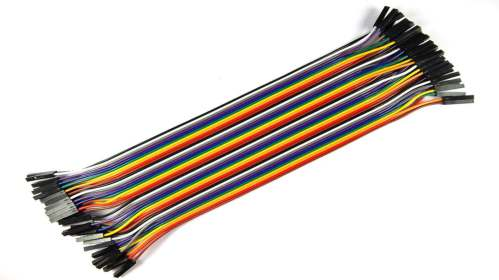
\includegraphics[width=3.46667in,height=1.95in]{media/8.jpg}

\textbf{4. Proposed System}

\textbf{4.3 DETAILS OF SOFTWARE}

{Visual Studio Code}: Visual Studio Code, also commonly referred to as
VS Code, is a source-code editor made by Microsoft with the Electron
Framework, for Windows, Linux, and macOS.


\includegraphics[width=1.49306in,height=1.49306in]{media/9.bmp}

Features include support for debugging, syntax highlighting, intelligent
code completion, snippets, code refactoring, and embedded Git.

Users can change the theme, keyboard shortcuts, and preferences, and
install extensions that add additional functionality.

{Thonny}: Thonny is an integrated development environment for Python
that is designed for beginners.


\includegraphics[width=1.49306in,height=1.49306in]{media/10.bmp}

It supports different ways of stepping through the code, step-by-step
expression evaluation, detailed visualization of the call stack, and a
mode for explaining the concepts of references and heap.

\textbf{4. Proposed System}

\textbf{4.3 DETAILS OF SOFTWARE}

{Jupyter Notebook}: Jupyter Notebook (formerly IPython Notebook) is a
web-based interactive computational environment for creating notebook
documents. Jupyter Notebook is built using several open-source
libraries, including IPython, ZeroMQ, Tornado, jQuery, Bootstrap, and
MathJax.


\includegraphics[width=1.49306in,height=1.49306in]{media/11.jpg}

A Jupyter Notebook document is a browser-based REPL containing an
ordered list of input/output cells which can contain code, text (using
Markdown), mathematics, plots and rich media. Underneath the interface,
a notebook is a JSON document, following a versioned schema, usually
ending with the ".ipynb" extension.

{Github}: GitHub, Inc. is an Internet hosting service for software
development and version control using Git.


\includegraphics[width=1.49306in,height=1.49306in]{media/12.jpg}

It provides the distributed version control of Git plus access control,
bug tracking, software feature requests, task management, continuous
integration, and wikis for every project. Headquartered in California,
it has been a subsidiary of Microsoft since 2018.

\textbf{4. Proposed System}

\textbf{4.4 Methodology}

\textbf{4.4.1 RESEARCH \& SURVEY}

The ``National Blindness and Visual Impairment Survey 2015-2019'' was
conducted to provide evidence about the present status of blindness and
visual impairment in India. The survey was planned by the Ministry of
Health and Family Welfare, Government of India. Dr. Rajendra Prasad
Centre for Ophthalmic Sciences, AIIMS, New Delhi was responsible for
planning and executing the fieldwork, monitoring, analysis, and report
writing of the survey.

{Results}:

\begin{itemize}
\item
  \begin{quote}
  Blindness was higher among illiterates (3.23\%) compared to the
  literate population. It was only 0.43\% among the 10th pass and above.
  \end{quote}
\item
  \begin{quote}
  Maximum prevalence of blindness was seen in 80+ age group (11.6\%),
  followed by 70-79 age group (4.1\%), 60-69 age group (1.6\%) and 50-59
  age group (0.5\%).
  \end{quote}
\item
  \begin{quote}
  Important barriers were financial constraints (22.1\%), the need for
  surgery not felt (18.4\%), and fear of surgery (16.1\%). Among males,
  the most important barriers were financial constraints (31.0\%) and
  local reasons (21.5\%). Among females, local reasons (23.1\%) and
  financial constraints (21.2\%) were the most important barriers.
  \end{quote}
\end{itemize}

\textbf{4. Proposed System}

\textbf{4.4 Methodology}

\textbf{4.4.2 BLOCK DIAGRAM}

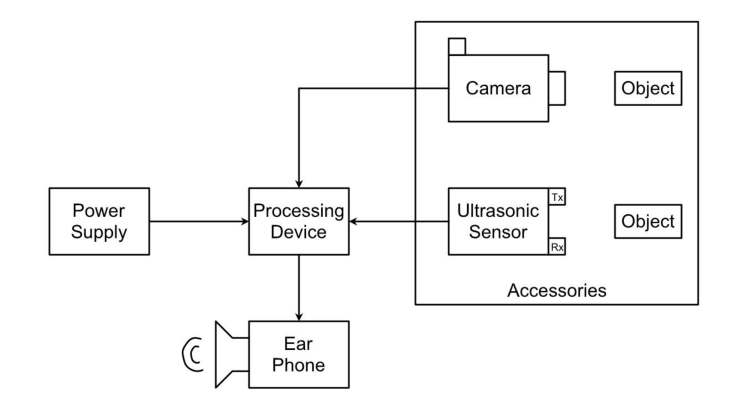
\includegraphics[width=5.12222in,height=2.85625in]{media/13.jpg}

The block diagram consists of the camera unit, sensor unit, processing
unit, power, and output unit.

{Camera Unit}: The camera unit is responsible for capturing images.

{Sensor Unit}: the sensor unit provides the distance of the object from
the unit.

{Processing Unit}: It plays an important role in detecting and
identifying objects (image processing), it also receives data from the
ultrasonic sensor and then instructs the user about the object
identified and the distance it is located at (So the user can navigate
accordingly).

{Output Unit}: The output is provided to a user in terms of an audio
signal using earphones.

\textbf{4. Proposed System}

\textbf{4.4 Methodology}

\textbf{4.4.3 FLOW CHART}

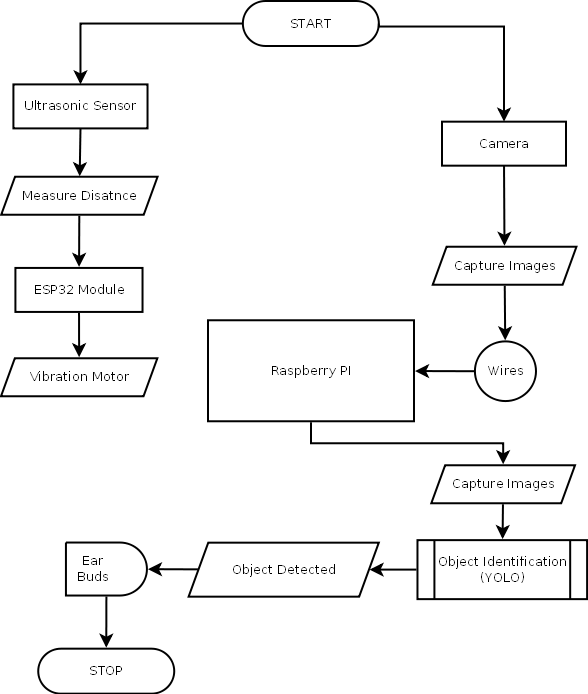
\includegraphics[width=4.96111in,height=5.85556in]{media/14.bmp}

\textbf{4. Proposed System}

\textbf{4.4 Methodology}

\textbf{4.4.4 OUTPUT}

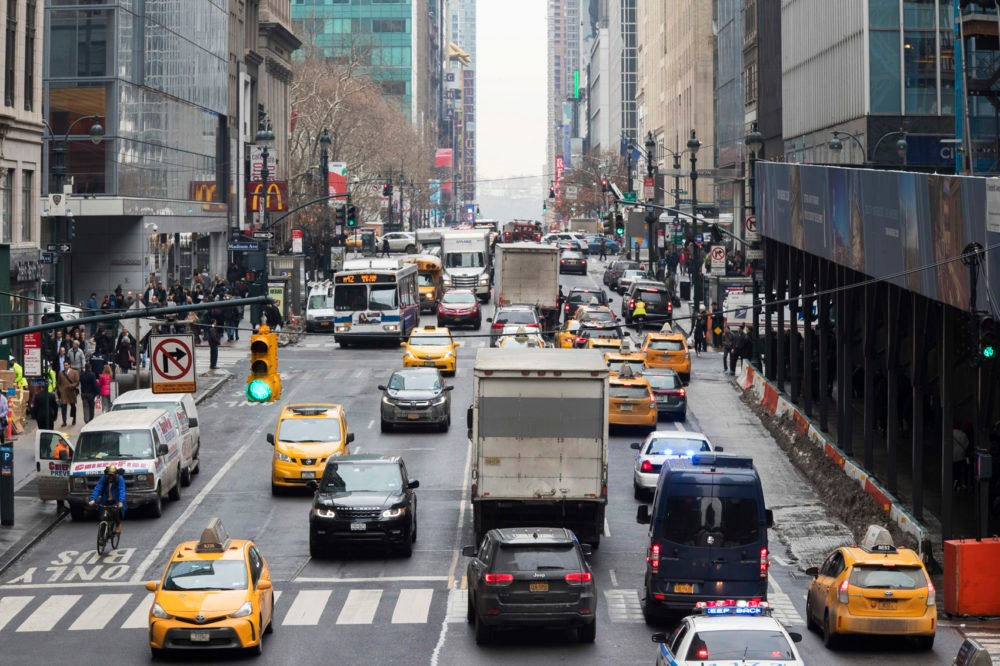
\includegraphics[width=5.41667in,height=3.60764in]{media/15.jpg}

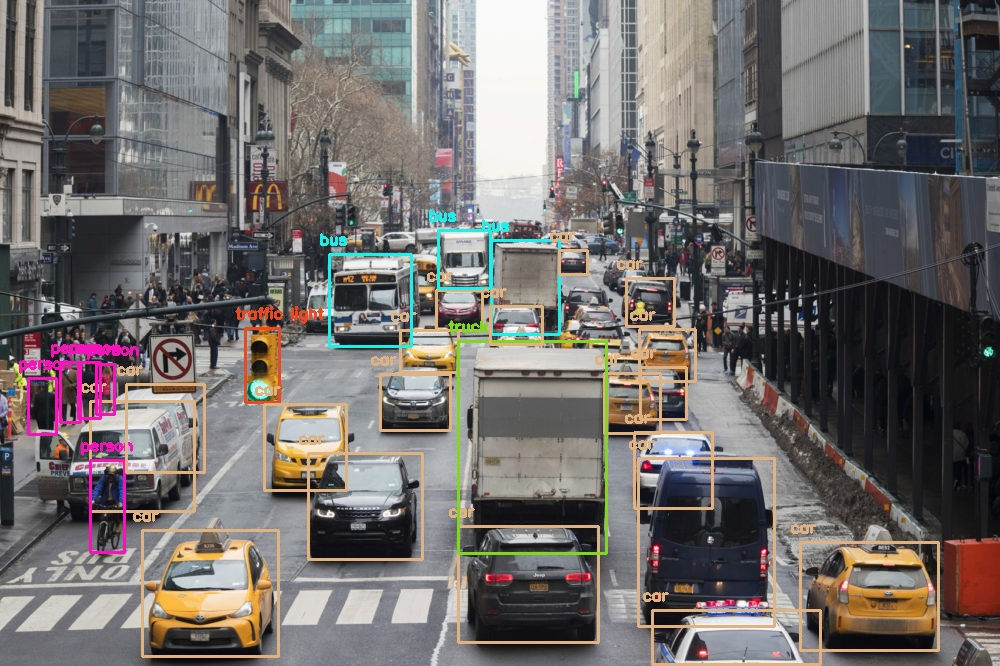
\includegraphics[width=5.41667in,height=3.60764in]{media/16.jpg}

Github: {https://github.com/mandarnaik016/YOLO-for-NAVI}

\textbf{5. IMPLEMENTATION PLAN FOR NEXT SEMESTER}

Once we are done with the simulation part, we will shift to implementing
the actual prototype of it. In this process, we will try to make the
project affordable so that the project becomes cost-effective and budget
friendly. Also, we may contact a visually impaired person to know
his/her needs and requirements.

Every time we will try to implement it in the real environment to get
the ideal output. After implementation, with the help of a visually
impaired person, we can test it in actual surroundings and can go
through their problems, and can improve the system simultaneously.

\textbf{6. CONCLUSION}

Visually impaired people faced many problems in their daily life, and
while traveling they always depend on any person or guide dog. Blind
Stick is very helpful for them but Stick has certain restrictions. We
created a navigation device for visually impaired people so that they
can perform their daily tasks.

There are certain Devices already available in the market but they
cannot solve the actual problem. Our project is an integrated system of
those devices.

In this paper, We present wearable Accessories in the form of Smart
Glasses and Smart Shoes for visually impaired people to deal with their
Tasks. Smart Glasses Capture images in front of those objects and
recognize them and convert it into an audio form which is then sent to
the earphones.

Once, a person goes close to that object Smart Shoes Gives output in the
form of a vibration motor so that the person avoids those objects. So,
with the help of this project person can easily detect and avoid an
obstacle, and also simply communicate with the environment.

\textbf{6. CONCLUSION}

\textbf{6.1 ADVANTAGES}

\begin{enumerate}
\def\labelenumi{\arabic{enumi}.}
\item
  \begin{quote}
  Both indoor and outdoor navigation are possible with the device.
  \end{quote}
\item
  \begin{quote}
  Detects obstacles and notifies the blind person through vibration and
  speech production.
  \end{quote}
\item
  \begin{quote}
  The devices placed are comfortable and easy to handle.
  \end{quote}
\item
  \begin{quote}
  Cheap, light-weight constructions available, effectively informs of
  obstacles at ground-level.
  \end{quote}
\end{enumerate}

\textbf{6.2 LIMITATIONS}

\begin{enumerate}
\def\labelenumi{\arabic{enumi}.}
\item
  \begin{quote}
  Does not protect from obstacles at the torso.
  \end{quote}
\item
  \begin{quote}
  The system is capable of identifying obstacles at reasonable distances
  and speeds; however, it is suggested that if an automated navigation
  system can be combined with a white cane, one can have a safe and
  reliable mobility aid.
  \end{quote}
\item
  \begin{quote}
  It needs many components that make the system complex and expensive.
  \end{quote}
\end{enumerate}

\textbf{6.3 FUTURE SCOPE}

\begin{enumerate}
\def\labelenumi{\arabic{enumi}.}
\item
  \begin{quote}
  This project can be extended by incorporating a GPS module.
  \end{quote}
\item
  \begin{quote}
  We can interface this module to send messages to near and dear once of
  the blind person regarding his/her current position.
  \end{quote}
\item
  \begin{quote}
  During so, we can track the moment of the blind person in a very
  efficient manner.
  \end{quote}
\item
  \begin{quote}
  The future work can be performance of the stick can be improved by
  adding health monitoring features.
  \end{quote}
\item
  \begin{quote}
  The proposed system must work on Wide Area Network and visually
  impaired people must be able to travel anywhere without restricting
  the areas.
  \end{quote}
\end{enumerate}

\textbf{7. REFERENCES}

\begin{enumerate}
\def\labelenumi{\arabic{enumi}.}
\item
  \begin{quote}
  Nishajith.A, Nivedha.J, Shilpa.S.Nair \& Prof. Mohammed Shaffi.J,
  ``SMART CAP -- WEARABLE VISUAL GUIDANCE SYSTEM FOR BLIND'',
  ISBN:978-1-5386-2456-2.
  \end{quote}
\item
  \begin{quote}
  Arjun Pardasani, Prithviraj N Indi, Sashwata Banerjee, Aditya Kamal \&
  Vaibhav Garg, ``Smart Assistive Navigation Devices for Visually
  Impaired People'', ISBN:978-1-7281-1322-7.
  \end{quote}
\item
  \begin{quote}
  Joe Louis Paul I, Sasirekha S, Mohanavalli S, Jayashree C, Moohana
  Priya P \& Monika K, ``Smart Eye for Visually Impaired-An aid to help
  the blind people'', ISBN:978-1-5386-9471-8.
  \end{quote}
\item
  \begin{quote}
  N.Loganathan, K.Lakshmi, N.Chandrasekaran, S.R.Cibisakaravarthi,
  R.Hari Priyanga \& K.HarshaVarthini, ``Smart Stick For Blind People'',
  ISBN:978-1-7281-5197-7.
  \end{quote}
\item
  \begin{quote}
  J. Bai, S. Lian, Z. Liu, K. Wang \& D. Liu, ``Smart guiding glasses
  for visually impaired people in indoor environment'', IEEE
  Transactions on Consumer Electronics, vol. 63, no. 3, pp. 1057-1062,
  2017.
  \end{quote}
\end{enumerate}

\end{document}
